\chapter{Task 2}
\begin{itemize}
   \item Man könnte den "Command" entwurfsmuster für Unser Projekt einsetzen, weil Kommandos an der Datenbank geschickt werden und diese fehlschlagen oder zu lange dauern können. Es wäre somit sinnvoll diese als Objekte zu speichern sodass man die Änderungen der Kommandos an der Datenbank rückgängig machen könnte wenn das Kommando abgebrochen wird oder fehlschlägt. Der "Command" entwurfsmuster löst das Problem Aktivitäten/Commandos wie Daten zu behandeln indem es die Aktivitäten/Commandos in Objekte verpackt mit einem gleichbleibenden Interface. Und das erlaubt es auch diese Kommandos rückgänig zu machen weil die verschiedenen Kommando Objekte auch die Daten speichern können die verändert werden um sie nach Bedarf wiederherzustellen.
   \item Das "Command" Muster Quelle: Vorlesung
   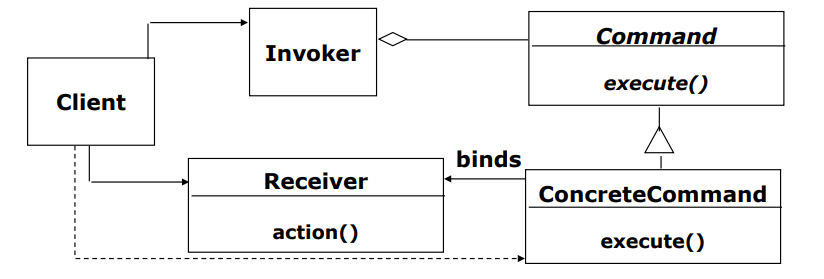
\includegraphics[width=\textwidth]{Immagini/b.jpg}
   \item Das "Command" Muster Angewendet
   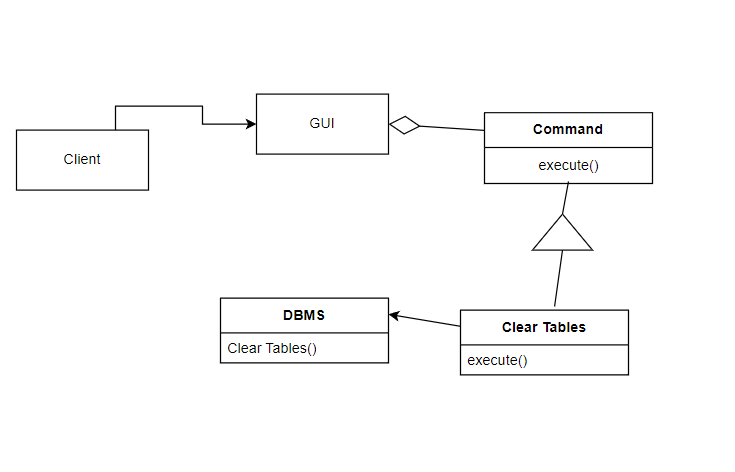
\includegraphics[width=\textwidth]{Immagini/a.jpg}
   \item Pseudo Code Für das Entwurfsmuster: 
   \lstinputlisting[language=java, frame=trBL]{
   class Gui{
	Command  clear_command; 
	void Init(){
		clear_command = new ClearTables()
	}
	void OnClickClearTable(){
		clear_command.execute()
	}
}
Interface Command{
	void exectue()
}
class table{
	int id;
	char data[1000];
}
class DBMS{
	void cleartables(List<table>){...}
	List< table> getalltables(){...}
}
class cleartables{
	List<tables> old_tables;
	@override
	execute(){
		old_tables = DBMS.getalltabels()
		DBMS.cleartables(DBMS.getalltabels())
	}
}
}

\end{itemize}
